\section{Types of convergence}

In probability theory there are several different notions of convergence and in
this section we will define and relate them.

\begin{mdframed}[innertopmargin=0pt]
\begin{definition}[Types of Convergence]
    \label{def: types of convergence}
    A sequence of random variables \((X_n)_{n\in \nat}\) in a normed
    space \((\domain, \norm{\cdot})\) converges to a random variable \(X\)
    \begin{itemize}
        \item \textbf{almost surely}, or \textbf{with probability one}, denoted by \(X_n \overset{\as}\to X\), if
        \[
            \prob[\Big]{\lim_{n \to \infty} X_n = X} = 1.
        \]

        \item \textbf{in \(L^p\)} for \(p \geq 1\), denoted by \(X_n \overset{L^p}\to X\), if \(\E{\norm{X_n}^p} < \infty\) for all \(n\), \(\E{\norm{X}^p} < \infty\)
        and
        \[
            \lim_{n \to \infty} \E[\Big]{\norm{X_n - X}^p} = 0.
        \]

        \item \textbf{in probability}, denoted by \(X_n \overset{p}\to X\), if for all \(\epsilon > 0\)
        \[
            \lim_{n \to \infty} \prob[\big]{\norm{X_n- X} \ge \epsilon} = 0.
        \]

        \item \textbf{in distribution}, denoted by \(X_n \overset{d}\to X\), if
        it satisfies one of the following equivalent conditions (\textbf{Portemanteau theorem}):\nobreak
        \begin{enumerate}[label=(B.\arabic*),leftmargin=3em]
            \item\label{it: b.lip} For all \(f\colon \domain \to \real\) bounded, Lipschitz continuous we have \eqref{eq: fun convergence},
            \item\label{it: b.cont} For all \(f\colon \domain \to \real\) bounded, continuous we have \eqref{eq: fun
            convergence},
            \item\label{it: b.a.s. cont} For all \(f\colon \domain \to \real\) bounded, measurable, almost surely
            continuous in \(X\), that is \(\prob[\big]{f\text{
            continuous in }X} = 1\), we have \eqref{eq:
            fun convergence}.
        \end{enumerate}
        Where \eqref{eq: fun convergence} is given by
        \begin{equation}
            \label{eq: fun convergence}\tag{B}
            \lim_{n\to\infty}\E{f(X_n)} = \E{f(X)}.
        \end{equation}
        \begin{enumerate}[label=(S.\arabic*), nosep,leftmargin=3em]
            \item\label{it: s.closed} For all \underline{closed} sets \(A\) we have
            \[\limsup_{n\in \nat} \prob{X_n \in A} \le \prob{X \in A}.\]
            \item\label{it: s.open} For all \underline{open} sets \(O\) we have 
            \[\liminf_{n\in \nat }\prob{X_n \in O} \ge \prob{X \in O}.\]
            \item\label{it: s.zero boundary} For all \underline{measurable} sets \(B\) with \underline{\(\prob{X \in \partial B} = 0\)} we have
            \[
                \lim_{n \to \infty} \prob{X_n \in B} = \prob{X \in B}.
            \]
        \end{enumerate}
        If \(\domain = \real\) the following condition is also equivalent:
        \begin{enumerate}[label={(DF)},nosep,leftmargin=3em]
            \item\label{it: df} \textbf{Convergence of distribution functions}:
            for all \(x \in \real\) satisfying \(\prob{X = x} = 0\),
            \[
                \lim_{n \to \infty} \prob{X_n \leq x} = \prob{X \leq x}.
            \]
        \end{enumerate}
    \end{itemize}
    We say that two random variables \(X\) and \(Y\) are \textbf{almost surely equal},
    denoted by \(X \overset{\as}= Y\), if \(\prob{X = Y} = 1\).
    The limit \(X\) of a convergent sequence of random variables \((X_n)_{n\in \nat}\) is \textbf{almost
    surely unique}, if
    \[
        X_n \overset{(\cdot)}\to X \quad \text{and} \quad X_n \overset{(\cdot)}\to Y \implies X \overset{\as}= Y.
    \]
\end{definition}
\end{mdframed}

\begin{remark}[Generalization to metric spaces]
    Except for convergence in \(L^p\), the definitions may be extended in the
    obvious way to metric spaces \((\domain, \metric)\). We
    prove the Portemanteau theorem in this generalized setting.
\end{remark}

While the Portemanteau theorem may seem like it introduces many different
definitions, there are essentially just \textbf{two} equivalent concepts:
The first is \textbf{convergence of bounded functions in expectation} \eqref{eq: fun
convergence}, where the functions have different degrees of continuity. 
This is useful as it is sufficient to prove convergence for the smallest
class of Lipschitz functions to conclude convergence for the larger classes.
The second big concept is that the \textbf{probabilities of sets converge},
with the caveat that probability mass may converge outside the set at the boundary
of the set. As an example consider the deterministic sequence \(\prob{X_n =
\frac1n} =1\). Then we have \(\prob{X_n \in (0,1]} =1\) for all \(n\) but for
the limit \(X\) we have \(\prob{X = 0} = 1\).
Thus open sets may lose probability mass at the boundary, while closed sets
may gain probability mass at the boundary. If the boundary has zero mass
in the limit however, then the probabilities converge.
The convergence of distribution functions is just a special case, since
\[
    \prob{X_n \le x} = \prob{X_n \in (-\infty, x]}.
\]
So we simply consider the sets \((-\infty, x]\) for all \(x\in \real\)
for which the boundary \(\{x\}\) has zero probability mass in the limit.
The interesting thing about this special case is that it is enough to check
convergence on this small family of sets to conclude convergence of
a much larger family of sets.

With convergence in distribution reduced to these two big concepts
let us contextualize the other types of convergence before we get lost in the details of the proof
of the Portemanteau theorem. We summarize the implications
between the different types of convergence in the following theorem.
Notice the fundamental difference between convergence in distribution and the
other, stronger, types of convergence that have almost surely unique limits. To
see that convergence in distribution cannot have almost surely unique limits,
consider the fact that \(X\) and \(-X\) have the same distribution when the
distribution of \(X\) is symmetric (Exercise \ref{ex: unique stochastic limits}
\ref{it: non-unique limits convergence in dist}).

\begin{theorem}[Convergence implications]
    \label{thm: convergence implications}
    For a sequence of random variables \((X_n)_{n\in\nat}\) and a
    random variable \(X\) the following implications hold:
    \begin{center}
        \begin{tikzcd}[
    every matrix/.append style={name=m},
    cells={nodes={
        draw, 
        rectangle, 
        rounded corners, 
        align=center, 
        minimum width=2.5cm, 
        minimum height=0.8cm,
        inner sep=5pt
    }},
    % 2. Spacing between nodes
    row sep=0.7cm,
    column sep=1.7cm,
    % 3. Global Arrow Styling
    execute at end picture={
        \draw[dashed, thick, gray] 
        ($(m-1-2.north east)!0.5!(m-1-3.north west) + (0.1, 1.2)$) -- 
        ($(m-1-2.south east)!0.5!(m-1-3.south west) + (0.1, -2.3)$)
        node[midway, fill=white, text=gray, font=\footnotesize, xshift=-32,yshift=-53] {\(X\) a.s.\ unique};
    }
]
    % --- Row 1 ---
    |[yshift=20]| \(X_n \overset{\as}\to X\)
    % \parbox{2.1cm}{Almost sure convergence}
    \arrow[r, Rightarrow, out=0, in=170]{}{\text{\ref{it: as to p}}}
    \arrow[d,xshift=20]{}[left]{\substack{\text{MCT/DCT}\\\text{(Measure Theory)}}}
    & \(X_n \overset{p}\to X\)
    \arrow[r, Rightarrow] {}[xshift=-4]{\ref{it: p to d}}
    \arrow[l, out=180, in=352, looseness=1] {}[below,yshift=-5]{\substack{\text{Borel-Cantelli}\\Sec.~\ref{sec: borel cantelli}}}
    \arrow[ld, out=250, in=358] {} [right,xshift=4,yshift=-5]{\substack{\text{\(X_n,X\) bounded}\\\text{(Exercise \ref{ex: p to Lp when bounded})}}}
    & \(X_n \overset{d}\to X\)
    \arrow[l, out=220, in=345, looseness=1] {}[below,xshift=19]{X \overset{\as}= c \in \real \text{ \ref{it: d to p}}}
    \arrow[ll, out=140, in=50, looseness=0.3]{}[above]{\text{Skorokhod (Exercise \ref{ex: skorokhod representation})}}

    \\
    % --- Row 2 ---
    % The loop is defined here on the Lp node
    \(\;X_n \overset{L^p}\to X,\; p \ge 1\)
    \arrow[ur, Rightarrow, out=5, in=230] {}[above]{\text{\ref{it: L1 to p}}}
    \arrow[loop below, Rightarrow, looseness=3.5, out=220, in=290,xshift=-10]{}[xshift=15,yshift=-3]{L_q \overset{\ref{it: Lq to Lp}}\implies L_p \; (p \le q)}
    % & $L^1$ \text{ convergence} \arrow[u, Rightarrow] {} {\text{\ref{it: L1 to p}}}
\end{tikzcd}
    \end{center}
    \begin{enumerate}[label=(\arabic*),noitemsep]
        \item\label{it: as to p}
        If \(X_n \xrightarrow{\as} X\), then \(X_n \xrightarrow{p} X\).
        \item\label{it: p to d}
        If \(X_n \xrightarrow{p} X\), then \(X_n \xrightarrow{d} X\).
        \item \label{it: d to p}
        If \(X\) is deterministic, i.e.\ \(X \overset{\as}= c\in \real\), then
        \(X_n \xrightarrow{d} X\) implies \(X_n \xrightarrow{p} X\).
        \item\label{it: Lq to Lp}
        If \(X_n \xrightarrow{L^q} X\) for some \(q \ge p \ge 1\), then \(X_n \xrightarrow{L^p} X\).
        \item\label{it: L1 to p}
        If \(X_n \xrightarrow{L^1} X\), then \(X_n \xrightarrow{p} X\).
    \end{enumerate}
    See Exercises \ref{ex: convergence in distribution but not in probability},
    \ref{ex: convergence in probability but not in Lp}, \ref{ex: convergence in
    Lp but not as} and \ref{ex: as but not Lp} for counterexamples showing that
    we have not forgotten any true implications.
    \begin{enumerate}[label=(\arabic*),noitemsep, resume]
        \item\label{it: uniqueness of limits}
        The limits of convergence in probability are almost surely unique.
        Consequently, the same holds for stronger notions of convergence.
    \end{enumerate}
\end{theorem}

Observe that it is not possible to conclude convergence in probability 
from convergence in distribution if the limit is not almost surely constant.
Indeed, if the limit \(X\) is non-deterministic it can have different values.
It is therefore possible to construct two independent random variables \(X\) and \(Y\)
with the same distribution by essentially ``shuffling'' the outcomes and
letting \(X\) take a different value from \(Y\) since there are multiple
options. Since the limit is then not unique we cannot have convergence in
probability.

The remainder of this section is structured as follows: First, we will introduce
a few easy to prove tools. We will use them to prove the convergence implication
(Theorem \ref{thm: convergence implications}) but we will use these tools in other
sections as well. After proving these tools it is then natural to prove
Theorem \ref{thm: convergence implications} after which we will finally get
back to proving the Portemanteau theorem.

The first tool we introduce is the Markov inequality. It will become a very
close friend of ours as we will make frequent use of it (or its corollary)
in the following sections. It may be the most used inequality in probability
theory.

\begin{mdframed}[innertopmargin=0pt]
\begin{theorem}[Markov inequality]
    \label{thm: markov inequality}
    For an interval \(I\subseteq \real\) let \(h\colon I\to (0, \infty)\) be a
    non-decreasing function and \(X\) an \(I\)-valued random variable.
    Then for all \(t \in I\) we have
    \[
        \prob{X \ge t} \le \frac{\E{h(X)}}{h(t)}.
    \]
\end{theorem}
\begin{corollary}[Chebyshev inequality]
    \label{cor: markov inequality Lp}
    Let \(X\) be a random variable in a normed space \((\domain, \norm{\cdot})\)
    with \(\E{\norm{X}^p} < \infty\) for some \(p \ge 1\). Then
    \[
        \prob[\Big]{\norm{X - \E{X}} \ge t}
        \le \frac{\E[\Big]{\norm[\big]{X-\E{X}}^p}}{t^p}
        \qquad \text{for all }t > 0.
    \]
\end{corollary}
\end{mdframed}
\begin{remark}[Historical note]
    The case \(p=2\) is the classical ``Chebyshev inequality'', which
    is older than Markov's inequality.  Markov was Chebyshev's student and the
    classical ``Markov inequality'' is the one from Theorem \ref{thm: markov
    inequality} with \(h(x) = x\). The generalizations above are best known
    as Markov's inequality but also referred to as Chebyshev's inequality by
    some authors. We try to compromise with the Corollary covering a
    special case.
\end{remark}

\begin{proof}[Proof of Corollary \ref{cor: markov inequality Lp}]
    Markov inequality applied to \(\tilde X = \norm{X - \E{X}}\) 
    and \(h(x) = x^p\) with \(I = [0, \infty)\).
\end{proof}

\begin{proof}[Proof of Theorem \ref{thm: markov inequality}]
    Since \(h\) is non-decreasing and \(t, X \in I\)
    we have that \(X \ge t\) implies \(h(X) \ge h(t)\)
    and thus
    \[\begin{aligned}
        \prob{X \ge t}
        &\le \prob[\big]{h(X) \ge h(t)}
        = \E{\ind{h(X) \ge h(t)}}
        \le \E[\Big]{\frac{h(X)}{h(t)}\ind{h(X) \ge h(t)}}
        \\
        &\le \E[\Big]{\frac{h(X)}{h(t)}},
    \end{aligned}
    \]
    where we have used \(h > 0\) in the last inequality to remove the indicator.
\end{proof}

Before we get to the proof of Theorem \ref{thm: convergence implications}
we introduce another Lemma. A special case of the Lemma is the proof that
convergence in probability implies convergence in distribution but we will use
this more general form for the continuous mapping results (Section \ref{sec:
continuous mapping}).

\begin{lemma}\label{lem: moving target p to d}
    Let \((X_n)_{n\in \nat}\) and \((Y_n)_{n\in \nat}\) be two sequences of
    random variables in the metric space \((\domain, \metric)\) and
    \(f\colon \domain \to \real\) a bounded, Lipschitz continuous function, then
    \[
        \metric(X_n,Y_n) \overset{p}\to 0
        \quad\implies\quad
        \abs[\big]{\E{f(X_n)} - \E{f(Y_n)}} \to 0.
    \]
\end{lemma}

\begin{proof}
    Since \(f\) is bounded we have that \(\abs{f(x)} \le M\) for all \(x\in
    \domain\) for some \(M > 0\). Let \(L\) further be the Lipschitz constant
    of \(f\) and choose an arbitrary \(\epsilon > 0\).
    Then
    \[\begin{aligned}
        &\abs{\E{f(X_n)} - \E{f(Y_n)}}
        \\
        &\le \E{\abs{f(X_n) - f(Y_n)}}
        \\
        &\le \E{\underbrace{\abs{f(X_n) - f(Y_n)}}_{\le L\metric(X_n, Y_n)} \ind{\metric(X_n, Y_n) \le \epsilon}}
        + \E{\underbrace{\abs{f(X_n) - f(Y_n)}}_{\le 2M} \ind{\metric(X_n, Y_n) > \epsilon}}
        \\
        &\le L \epsilon + 2M \underbrace{\prob{\metric(X_n, Y_n) > \epsilon}}_{\to 0}.
    \end{aligned}\]
    Using \(\metric(X_n, Y_n) \overset{p}\to 0\) we thus we have \(\limsup_{n\to
    \infty} \abs{\E{f(X_n)} - \E{f(Y_n)}} \le L \epsilon\)
    for arbitrary \(\epsilon > 0\) and thus its limit must be zero.
\end{proof}

\begin{proof}[Proof (Theorem \ref{thm: convergence implications})]
    We will prove all implications not involving \(L^p\) for metric spaces. You
    may assume \(\metric(x,y) = \norm{x-y}\) for the sake of simplicity.
    \begin{enumerate}[wide=0pt]
        \item[\ref{it: p to d}] To see that Lemma \ref{lem: moving target p to d}
        proves that convergence in probability implies convergence in distribution,
        choose \(Y_n = X\) and observe that by definition
        \[
            \metric(X_n, X) \overset{p}\to 0 \iff X_n \overset{p}\to X
        \]
        then this Lemma proves \ref{it: b.lip} from the Portemanteau theorem.

        \item[\ref{it: L1 to p}] Convergence in probability may be easily deduced
        from the \(L^1\) Chebyshev inequality (Corollary
        \ref{cor: markov inequality Lp}): We have for \(\epsilon > 0\) \[
            \prob[\big]{\norm{X_n - X} > \epsilon}
            \le \frac{\E[\big]{\norm{X_n - X}}}{\epsilon}
            \to 0.
        \]

        \item[\ref{it: as to p}] To prove that almost sure convergence implies convergence in 
        probability observe that the set of point-wise convergence is given by
        \begin{align*}
            \set{X_n \to X}
            &= \set[\Big]{\omega \in \Omega : \lim_{n \to \infty} X_n(\omega) = X(\omega)}
            \\
            \overset{\text{def.}}&= \set[\Big]{
                \omega \in \Omega
                : \forall \epsilon > 0, \exists N\in \nat, \forall n \ge N
                : \metric(X_n(\omega), X(\omega)) < \epsilon}.
            \\
            &= \bigcap_{\epsilon > 0} \bigcup_{N \in \nat} \bigcap_{n \ge N}
            \set[\Big]{\omega \in \Omega : \metric(X_n(\omega), X(\omega)) < \epsilon}.
        \end{align*}
        By de Morgan's laws for set complements and almost sure
        convergence we therefore have
        \begin{align*}
            0 &= \prob[\big]{X_n \not\to X}
            \\
            &= \prob[\bigg]{\bigcup_{\epsilon > 0} \bigcap_{N \in \nat} \bigcup_{n \ge N}
            \set[\Big]{\omega \in \Omega : \metric(X_n(\omega), X(\omega)) \ge \epsilon}}
            \\
            \overset{\text{fix } \epsilon}&\ge \prob[\bigg]{\bigcap_{N \in \nat} \bigcup_{n \ge N}
            \set[\Big]{\omega \in \Omega : \metric(X_n(\omega), X(\omega)) \ge \epsilon}}
            \\
            &= \lim_{N \to \infty} \prob[\Big]{\bigcup_{n \ge N}
            \set[\Big]{\omega \in \Omega : \metric(X_n(\omega), X(\omega)) \ge \epsilon}}
            \\
            \overset{\text{fix } n=N}&\ge \lim_{N\to \infty} \prob[\big]{\metric(X_N, X) \ge \epsilon},
        \end{align*}
        where the penultimate equality follows from the continuity of the
        probability measure
        \[
            \lim_{N\to \infty} \prob{A_N} = \prob[\big]{\bigcap_{N\in \nat} A_N}
        \] for a decreasing sequence of
        events \(A_1 \supseteq A_2 \supseteq \ldots\)
        \continuityOfMeasure.

        \item[\ref{it: d to p}] Assume that \(X\equiv c\in \domain\), choose any
        \(\epsilon>0\) and let \(\ball{c}{\epsilon}\) denote the
        \(\epsilon\)-ball centered at \(c\).
        Then its border has zero probability under the distribution of \(X\), that is
        \(\prob{X\in \partial\ball{c}{\epsilon}} = 0\).
        Using \ref{it: s.zero boundary} from the Portemanteau theorem
        this implies
        \[
            \prob[\big]{\metric(X_n,X) < \epsilon}
            = \prob[\big]{X_n \in \ball{c}{\epsilon}}
            \to \prob[\big]{X \in \ball{c}{\epsilon}} = 1.
        \]
        Consequently \(\prob[\big]{\metric(X_n, X) \ge \epsilon} \to 0\).

        

        \item[\ref{it: Lq to Lp}] We will prove this implication in a separate
        section on \(L^p\) spaces (see Remark \ref{rem: Lp convergence} in
        Section \ref{sec: Lp spaces}).

        \item[\ref{it: uniqueness of limits}] See Exercise \ref{ex: unique stochastic limits}.
        \qedhere
    \end{enumerate}
\end{proof}

What remains is to prove the Portemanteau theorem as we have already made
use of different variants of convergence in distribution to prove the convergence
implications above.

\begin{myproof}[Proof (Portemanteau Theorem)]
    The proof strategy is as follows:
    \begin{center}
            \begin{tikzcd}[
        column sep=.6cm,
        row sep=0.5cm,
    ]
        \ref{it: b.a.s. cont}
        \arrow[r, Rightarrow]{}{\text{trivial}}
        & \ref{it: b.cont}
        \arrow[r, Rightarrow]{}{\text{trivial}}
        & \ref{it: b.lip}
        \arrow[r, Rightarrow]{}{!}
        & \ref{it: s.closed}
        \arrow[r, Leftrightarrow]{}{\text{easy}}
        & \ref{it: s.open}
        \arrow[r, Rightarrow]{}{\text{easy}}
        & \ref{it: s.zero boundary}
        \arrow[r, Rightarrow]{}{!}
        \arrow[d, Rightarrow]{}{\text{trivial}}
        & \ref{it: b.a.s. cont}.
        \\
        & & & & & \ref{it: df}
        \arrow[ul, Rightarrow]{}{!}
    \end{tikzcd}
    \end{center}
    The equivalence of \ref{it: s.open} and \ref{it: s.closed} follows from
    directly from set complements. These two conditions then imply \ref{it: s.zero boundary}
    by considering the interior and closure of the set \(B\) for an upper and lower
    bound.
    % Specifically, we have that \(\prob{X \in \closure{B}} = \prob{X \in B} = \prob{X\in \interior{B}}\)
    % as \(\prob{X \in \partial B} = 0\). This implies
    % \[\begin{aligned}
    %     \prob{X \in B} = \prob{X \in \interior{B}}
    %     &\le \liminf_{n\to \infty} \prob{X_n \in \interior{B}}
    %     \\
    %     &\le \lim_{n\to\infty} \prob{X_n \in B}
    %     \\
    %     &\le \limsup_{n\to \infty} \prob{X_n \in \closure{B}}
    %     \le \prob{X \in \closure{B}} = \prob{X \in B}.
    % \end{aligned}
    % \]

    % \begin{wrapstuff}[type=figure,width=.35\textwidth,top=1]
    %     \scalebox{0.7}{
    %     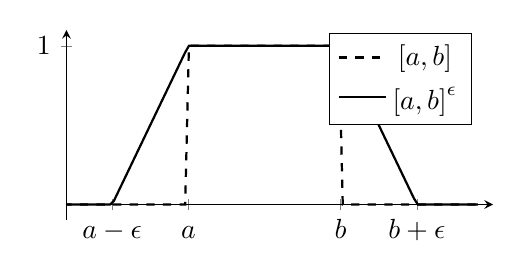
\begin{tikzpicture}
    \begin{axis}[
        axis lines=middle,
        xmin=0.2, xmax=3,
        ymin=-0.1, ymax=1.1,
        samples=200,
        domain=-2:2.9,
        width=7cm,
        height=4cm,
        legend style={at={(0.95,.5)}, anchor=south east},
        xtick={0.5, 1, 2, 2.5},
        ytick={0,1},
        xticklabels={\(a-\epsilon\), \(a\), \(b\), \(b+\epsilon\)},
        xticklabel style={text height=1.5ex}
    ]

    % Indicator function
    \addplot[
        thick,
        dashed
    ] {x <= 1 ? 0 : (x>2 ? 0: 1)};
    \addlegendentry{$\ind{[a,b]}$}

    % Lipschitz approximation
    \addplot[
        thick
    ] {
        x <= 0.5 ? 0 :
        (x >= 2.5 ? 0: 
        (x < 1 ? 2*(x-0.5) : 
        (x > 2 ? -2*(x-2) + 1 : 1)
        )
        )
    };
    \addlegendentry{$\ind{[a,b]}^{\vphantom{(}\epsilon}$}

    \end{axis}
\end{tikzpicture}
    %     }
    % \end{wrapstuff}

    \begin{wrapfigure}[5]{o}{0.35\textwidth}
        \scalebox{0.7}{
        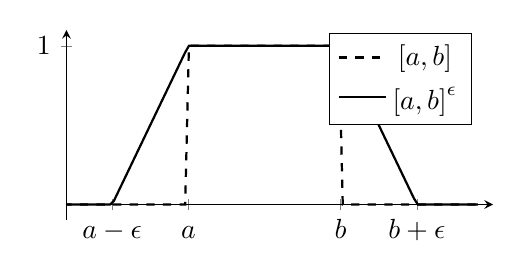
\begin{tikzpicture}
    \begin{axis}[
        axis lines=middle,
        xmin=0.2, xmax=3,
        ymin=-0.1, ymax=1.1,
        samples=200,
        domain=-2:2.9,
        width=7cm,
        height=4cm,
        legend style={at={(0.95,.5)}, anchor=south east},
        xtick={0.5, 1, 2, 2.5},
        ytick={0,1},
        xticklabels={\(a-\epsilon\), \(a\), \(b\), \(b+\epsilon\)},
        xticklabel style={text height=1.5ex}
    ]

    % Indicator function
    \addplot[
        thick,
        dashed
    ] {x <= 1 ? 0 : (x>2 ? 0: 1)};
    \addlegendentry{$\ind{[a,b]}$}

    % Lipschitz approximation
    \addplot[
        thick
    ] {
        x <= 0.5 ? 0 :
        (x >= 2.5 ? 0: 
        (x < 1 ? 2*(x-0.5) : 
        (x > 2 ? -2*(x-2) + 1 : 1)
        )
        )
    };
    \addlegendentry{$\ind{[a,b]}^{\vphantom{(}\epsilon}$}

    \end{axis}
\end{tikzpicture}
        }
        \caption{
            \(\epsilon\)-bump function example.
        }
    \end{wrapfigure}
    
    ``\ref{it: b.lip} \(\Rightarrow\) \ref{it: s.closed}'': We use \(\epsilon\)-bump
    functions as approximations of indicators.
    Specifically, using \(x_+ \coloneq \max\{x, 0\}\) we define
    \[
        \ind{A}^\epsilon(x) \coloneq \Bigl(1-\frac{\metric(x, A)}\epsilon\Bigr)_+,
    \]
    where the distance of \(x\) to the set \(A\) is
    defined as
    \[
        \metric(x,A) = \inf_{y\in A} \metric(x,y).
    \]
    Lipschitz continuity is straightforward to verify (Exercise \ref{ex: lipschitz bump functions}).
    Using an \(\epsilon\)-increase in size of the set \(A\)
    \[
        A_\epsilon \coloneq \set{x \in \domain : \metric(x,A) \le \epsilon}
        = A + \ball{0}{\epsilon},
    \]
    we have  \(\ind{A}(x) \le \ind{A}^\epsilon(x) \le \ind{A_\epsilon}(x)\) for all \(x\).
    Consequently we have for any closed set \(A\)
    \[\begin{aligned}
        \prob{X_n \in A} = \E{\ind{A}(X_n)}
        &\le \E{\ind{A}^\epsilon(X_n)}
        \\
        \overset{\ref{it: b.lip}}&\to \E{\ind{A}^\epsilon(X)} \le \E{\ind{A_\epsilon}(X)}
        = \prob{X \in A_\epsilon},
    \end{aligned}
    \]
    Thus for every \(\epsilon >0\) we have
    \(
        \limsup_{n\to \infty} \prob{X_n \in A} \le \prob{X \in A_\epsilon}.
    \)
    Since this is true for any \(\epsilon >0\) define
    \(B_m \coloneq A_{\frac1m}\), then we have
    \[
        \limsup_{n\to \infty} \prob{X_n \in A}
        \le \lim_{m\to\infty}\prob{X \in B_m}
        = \prob[\Big]{X \in \bigcap_{m\in \nat} B_m}
        = \prob{X \in A},
    \]
    where we recall that \(\lim_{N\to \infty}
    \prob{A_N} = \prob[\big]{\bigcap_{N\in \nat} A_N}\) for a decreasing
    sequence of events \(A_1 \supseteq A_2 \supseteq \ldots\)
    \continuityOfMeasure,
    and \(B_m \supseteq B_{m+1} \supseteq \dots\) with \(\bigcap_{m\in \nat} B_m = A\).

    ``\ref{it: s.zero boundary} \(\Rightarrow\) \ref{it: b.a.s. cont}'': For the
    opposite direction it is necessary to discretize a bounded, measurable,
    almost surely continuous function \(f\colon \domain \to \real\). For this discretization we want to
    select a finite number of \(y_0 \le \ldots \le y_N\) in \(\real\)
    such that 
    \begin{enumerate}[noitemsep]
        \item the bounded range of \(f\) is contained in the interval \([y_0, y_N)\),
        \item the \(y_i\) are an \(\epsilon\)-grid, i.e.\ \(y_{i+1} - y_i < \epsilon\) for all \(i\),
        \item \(\prob{f(X) = y_i} = 0\) for all \(i\).
    \end{enumerate}
    That the first two conditions can be satisfied is trivial by the boundedness of \(f\). For
    the third condition we observe that the set of points that do not
    satisfy this condition is at most countable
    \[
        \set[\big]{y \in \real : \prob{f(X) = y} > 0}
        = \bigcup_{k=1}^\infty \underbrace{\set[\Big]{y \in \real : \prob{f(X) = y} \ge \tfrac1k}}_{\text{at most \(k\)-many}}.
    \]
    Since there is thus an uncountable number of choices left we may assume that
    the \(y_i\) satisfy all three conditions.

    The third condition implies for \(E_i = [y_{i-1}, y_i)\) that
    \(\prob{f(X) \in \partial E_i} = 0\). We will now prove that this
    implies \(\prob{X \in \partial f^{-1}(E_i)} = 0\), which will
    allow us to apply \ref{it: s.zero boundary} to the sets \(f^{-1}(E_i)\).
    Let \(D_f\) be the set of discontinuities of \(f\). Then for any set \(A\)
    we claim to have
    \begin{equation}
        \label{eq: boundary inclusion}    
        \partial f^{-1}(A) \subseteq f^{-1}(\partial A) \cup D_f.
    \end{equation}
    \begin{center}
    \begin{tabular}{|p{0.9\textwidth}}
    To see this, let \(x \in \partial f^{-1}(A)\). If \(x\in D_f\) we are done
    so assume that \(f\) is continuous in \(x\). By definition of continuity
    there exists for any \(\epsilon > 0\) a \(\delta > 0\) such that
    \(f(\ball{x}{\delta}) \subseteq \ball{f(x)}{\epsilon}\). By definition of
    the boundary, there exists
    \[
        y \in f^{-1}(A) \cap \ball{x}{\delta}
        \quad \text{and}\quad
        z \in \bigl(f^{-1}(A)\bigr)^\complement \cap \ball{x}{\delta}.
    \]
    Since \(\bigl(f^{-1}(A)\bigr)^\complement = f^{-1}(A^\complement)\) we consequently
    have
    \[
        f(y) \in A \cap \ball{f(x)}{\epsilon}
        \quad \text{and}\quad
        f(z) \in A^\complement \cap \ball{f(x)}{\epsilon}.
    \]
    As neither set may thus be empty for any \(\epsilon > 0\), we have that
    \(f(x) \in \partial A\) and thus \(x \in f^{-1}(\partial A)\).
    \end{tabular}
    \end{center}
    With \eqref{eq: boundary inclusion} we conclude
    \[
        \prob{ X \in \partial f^{-1}(E_i)}
        \le \underbrace{\prob[\big]{X \in f^{-1}(\partial E_i)}}_{=\prob{f(X) \in \partial E_i}} + \underbrace{\prob{X \in D_f}}_{=0} = 0.
    \]
    Finally, we may use the discretization we built. Observe that if \(f(X_n)
    \in E_i\), then \(f(X_n) \le y_i\). Since the sets \(E_i\) cover
    the range of \(f\) we have
    \[
        \E{f(X_n)}
        \le \E[\Big]{\sum_{i=1}^N y_i \ind{E_i}(f(X_n))}
        = \sum_{i=1}^N y_i \underbrace{\prob{X_n \in f^{-1}(E_i)}}_{\overset{\ref{it: s.zero boundary}}\to \prob{X \in f^{-1}(E_i)}}
    \]
    where we use \(\prob{X \in \partial f^{-1}(E_i)} = 0\). Using \(y_i \le f(X) +
    \epsilon\) for \(f(X) \in E_i\) we get
    \[
        \sum_{i=1}^N y_i \prob{X \in f^{-1}(E_i)}
        = \E[\Big]{\sum_{i=1}^N y_i \ind{E_i}(f(X))}
        \le \E{f(X)} + \epsilon.
    \]
    Put together this implies
    \[
        \limsup_{n\to \infty} \E{f(X_n)}
        \le \E{f(X)} + \epsilon.
    \]
    As this is true for any \(\epsilon >0\) we may drop it. Applying the same
    arguments to \(-f\) we obtain the lower bound and consequently
    \(\E{f(X_n)} \to \E{f(X)}\).

    ``\ref{it: df} \(\Rightarrow\) \ref{it: b.lip}'':
    Let \(F(x) = \prob{X\le x}\) and \(F_n(x) = \prob{X_n \le x}\) be the
    distribution functions of \(X\) and \(X_n\). We need to deduce from
    \(F_n(x) \to F(x)\) for all \(x\in \real\) with \(\prob{X = x} = 0\) that
    \[
        \E{f(X_n)} \to \E{f(X)}
    \]
    for all bounded, Lipschitz continuous functions \(f\colon \real \to \real\).
    If \(f\) has Lipschitz constant \(L\), then by considering \(\frac1L f\) and
    linearity of the expectation we may assume without loss of generality that
    \(L=1\). Similarly, we may assume it is bounded by \(1\). Let \(\epsilon > 0\) and choose \(N\) large enough that it is possible to choose
    \(y_0 < \ldots < y_N\) such that
    \[
        F(y_0) \le \epsilon,\quad F(y_N) \ge 1 - \epsilon,
        \quad\text{and}\quad
        y_{i+1} - y_i < \epsilon\quad  \text{ for all } i.
    \]
    There are only countably many points where \(\prob{X = y} \neq 0\),
    since the number of points where \(\prob{X=y} \ge \tfrac1m\) is finite and a
    countable union (over \(m\)) of finite sets is countable.  We may therefore
    choose \(y_i\) such that \(\prob{X = y_i} = 0\) for all \(i\).
    For all \(x\in (y_{i-1}, y_i]\) we then have
    \[
        \abs{f(x) - f(y_i)} \overset{1\text{-Lip}}\le \abs{x-y_i} < \epsilon,
    \]
    and thus \(f(x) \le f(y_i) + \epsilon \le f(x)\). Recall that \(f\) is moreover bounded
    by \(1\) such that
    \[\begin{aligned}
        \E{f(X_n)}
        &\le \E{\ind{X_n \le y_0}} + \E[\Big]{\sum_{i=1}^N (f(y_i) +\epsilon)\ind{(y_{i-1}, y_i]}(X_n)}
        + \E{\ind{X_n > y_N}}
        \\
        &\le F_n(y_0) + \sum_{i=1}^N (f(y_i) + \epsilon) (F_n(y_i) - F_n(y_{i-1})) + (1 - F_n(y_N))
    \end{aligned}
    \]
    Since \(\lim_{n\to \infty} F_n(y_i) = F(y_i)\) for all \(i\) we consequently have
    \[\begin{aligned}
        \limsup_{n\to \infty} \E{f(X_n)}
        &\le \underbrace{F(y_0)}_{\le \epsilon} + \sum_{i=1}^N (f(y_i) + \epsilon) (F(y_i) - F(y_{i-1})) + \underbrace{(1 - F(y_N))}_{\le \epsilon}
        \\
        &\le 2\epsilon + \E[\Big]{\sum_{i=1}^N \underbrace{(f(y_i) + \epsilon)}_{\le f(X) + 2\epsilon} \ind{(y_{i-1}, y_i]}(X)}
        \\
        &\le 4\epsilon + \E{f(X)} - \E{f(X) \ind{X \le y_0}} - \E{f(X) \ind{X > y_N}}
        \\
        &\le 6\epsilon + \E{f(X)}.
    \end{aligned}
    \]
    Since \(\epsilon>0\) was arbitrary we thus obtain \(\limsup_{n\to \infty}
    \E{f(X_n)} \le \E{f(X)}\). Applying the same arguments to \(-f\) we get the
    lower bound.
\end{myproof}


\subsection*{Exercises \thesection}

% counterexample: convergence in distribution but not in probability

\begin{exercise}[Convergence in distribution but not probability \Coffeecup]
    \label{ex: convergence in distribution but not in probability}
    Let \(X\) be a random variable with \(\prob{X=-1} = \frac12\) and \(\prob{X=1}=\frac12\).
    \[
        X_n \coloneq (-1)^n X
    \]
    Prove that
    \begin{enumerate}[label=(\alph*), noitemsep]
        \item \(X_n \xrightarrow{d} X\)
        \begin{solution}
            Observe that the distribution of \(X\) is symmetric, that is
            \[
                \prob{-X \le x} = \prob{X \le x} \qquad \forall x\in \real.
            \]
            Consequently, for any \(x \in \real\) we have \(\prob{X_n \le x} = \prob{X \le x}\).
            In particular this implies \(\prob{X_n \le x} \to \prob{X \le x}\) for all \(x\).
        \end{solution}

        \item \(X_n\) does not converge in probability to \(X\).
        \begin{solution}
            We have for \(\epsilon = 1\) and every odd \(n\)
            \[
                \prob{\abs{X - X_n} \ge \epsilon}
                = \prob{2\abs{X} \ge 1} = 1
            \]
            The sequence \(\prob{|X_n - X| \ge \epsilon}\) thus does not converge to \(0\).
        \end{solution}
    \end{enumerate}
\end{exercise}



\begin{exercise}[Convergence in probability but not \(L^p\) \Coffeecup]
    \label{ex: convergence in probability but not in Lp}
    Let \(U\sim \uniform(0,1)\) be a standard uniform random variable and define
    \[
        X_n \coloneq n \ind{[0, 1/n)}(U)
    \]
    Show that
    \begin{enumerate}[label=(\alph*), noitemsep]
        \item the sequence \((X_n)_{n\in \nat}\) converges to \(0\) in probability,
        \begin{solution}
            We have for any \(\epsilon > 0\)
            \[
                \prob{|X_n - 0| \ge \epsilon}
                \le \prob(X_n \neq 0)
                = \prob[\big]{U\le \tfrac1n}
                = \tfrac1n
                \to 0.
                \qedhere
            \]
        \end{solution}

        \item the sequence \((X_n)_{n\in \nat}\) does not converge to \(0\) in \(L^1\),
        \begin{solution}
            We have
            \[
                \E{|X_n - 0|}
                = \E{X_n}
                = n \cdot \prob[\big]{U \in [0, 1/n)}
                = n \cdot \frac1n
                = 1 \not\to 0.
                \qedhere
            \]            
        \end{solution}

        \item For every \(p \ge 1\) construct a sequence \((Y_n)_{n\in \nat}\) such that
        \(Y_n\xrightarrow{L^q} 0\) for all \(q < p\) but not for \(q \ge p\).
        \begin{solution}
            Define \(Y_n \coloneq X_n^{1/p}\) with \(X_n\) as above. Then
            \[
                \E{|Y_n - 0|^q} = \E{X_n^{q/p}} = n^{q/p} \cdot \prob[\big]{U \in [0, 1/n)} = n^{q/p - 1}.
            \]
            This converges to \(0\) for all \(q < p\) but not for \(q \ge p\).
        \end{solution}
        \end{enumerate}
\end{exercise}


\begin{exercise}[Convergence in \(L^p\) but not almost surely \Coffeecup\Coffeecup] 
    \label{ex: convergence in Lp but not as}
    Let \(U\sim \uniform(0,1)\) be a standard uniform random variable.
    We will scan the interval for \(U\) with increasingly fine measurements. Specifically,
    let
    \begin{alignat*}{7}
        X_1 &\coloneq \ind{[0,1)}(U)
        \\
        X_2 &\coloneq \ind{[0,\frac12)}(U)
        \quad & X_3 &\coloneq \ind{[\frac12, 1)}(U)
        \\
        X_4 &\coloneq \ind{[0, \frac14)}(U)
        \quad & X_5 &\coloneq \ind{[\frac14, \frac12)}(U)
        \quad & X_6 &\coloneq \ind{[\frac12, \frac34)}(U)
        \quad & X_7 &\coloneq \ind{[\frac34, 1)}(U)
    \end{alignat*}
    That is
    \[
        X_n \coloneq \ind{\left[
            \frac{k}{2^{m}}, \frac{k+1}{2^{m}}
        \right)}(U),
        \quad \text{with}\quad 
        m \coloneq \lfloor\log_2(n)\rfloor, \quad k \coloneq n - 2^m. 
    \]
    Show that
    \begin{enumerate}[label=(\alph*), noitemsep]
        \item\label{it: (conv in Lp but not as) in Lp}
        \(X_n \xrightarrow{L^p} 0\),

        \item\label{it: (conv in Lp but not as) in prob}
        \(X_n \xrightarrow{p} 0\),

        \item\label{it: (conv in Lp but not as) not as}
        \(X_n\) does not converge almost surely to \(0\).
    \end{enumerate}
\end{exercise}
\begin{solution}
\begin{enumerate}[wide=0pt]
    \item[\ref{it: (conv in Lp but not as) in Lp}]
    We have for any \(p \ge 1\)
    \[
        \E{|X_n|^p} = \int_0^1 \ind{
            \left[\frac{k}{2^{m}}, \frac{k+1}{2^{m}} \right)
        }(u) \, du
        = \frac{1}{2^m} = 2^{-\lfloor \log_2(n) \rfloor} \to 0.
    \]
    Consequently, \(X_n \xrightarrow{L^p} 0\).

    \item[\ref{it: (conv in Lp but not as) in prob}]
    \(X_n \xrightarrow{L^p} 0\) implies \(X_n \xrightarrow{p} 0\) by Theorem
    \ref{thm: convergence implications} \ref{it: L1 to p}.

    Alternatively:
    \[
        \prob[\bigl]{|X_n - 0| \ge \epsilon}
        = \prob{X_n = 1}
        = 2^{-\lfloor \log_2(n) \rfloor} \to 0.
    \]
    for any \(\epsilon \in (0,1]\) and \(\prob[\bigl]{|X_n - 0| \ge
    \epsilon}=0\) for \(\epsilon > 1\).

    \item[\ref{it: (conv in Lp but not as) not as}]
    Choose any \(\omega \in \set{U\in [0,1)}\). We will show that there exists an
    \(\epsilon > 0\), specifically any \(\epsilon < 1\) such that
    \(|X_n(\omega) - 0| \ge \epsilon\) for infinitely many \(n\).
    Since we show this for any \(\omega\in \set{U\in [0,1)}\), this would imply
    \[
        \prob{X_n \not\to 0} \ge \prob{U \in [0,1)} = 1.
    \]
    For any \(N\in \nat\) the task is consequently to find \(n\ge N\)
    such that \(X_n(\omega) = 1\). Let \(m \coloneq \lfloor \log_2(N) \rfloor + 1\).
    Then there exists a \(k \in \{0, \ldots, 2^m-1\}\) such that
    \[
        \frac{k}{2^m} \le U(\omega) < \frac{k+1}{2^m}.
    \]
    Consequently, for \(n = 2^m + k\) we have \(n \ge N\) and
    \[
        X_n(\omega) = \ind{\left[
            \frac{k}{2^{m}}, \frac{k+1}{2^{m}}
        \right)}(U(\omega)) = 1.
        \qedhere
    \]
\end{enumerate}
\end{solution}


\begin{exercise}[subtitle={Stochastic convergence sometimes implies \(L^p\) \Coffeecup}]
    \label{ex: p to Lp when bounded}
    Assume that \(X_n\) and \(X\) are bounded random variables. That is 
    \(\sup_n\|X_n\| \le c\) and \(\|X\|\le c\) with probability one for some \(c
    \in \real\). Show that then \(X_n \overset{p}\to X\) implies \(X_n
    \overset{L^p}\to X\).
    \begin{remark}
        This is a weak form of the dominated convergence theorem, where the constant
        is the dominating function.
    \end{remark}
\end{exercise}
\begin{solution}
    We have for every \(\epsilon > 0\)
    \[\begin{aligned}
        \E[\big]{\norm{X_n - X}^p}
        &= \E[\big]{\norm{X_n - X}^p \ind{\norm{X_n - X} < \epsilon}}
        + \E[\big]{\norm{X_n - X}^p \ind{\norm{X_n - X} \ge \epsilon}}
        \\
        &\le \epsilon^p + (2c)^p \prob[\big]{\norm{X_n - X} \ge \epsilon}.
    \end{aligned}
    \]
    Due to \(X_n \overset{p}\to X\) the second term converges to \(0\)
    and we thus have
    \[
        \limsup_{n\to \infty} \E[\big]{\norm{X_n - X}^p} \le \epsilon^p.
    \]
    Since this is true for any \(\epsilon > 0\) we have the claim.
\end{solution}


\begin{exercise}[Stochastic triangle inequality \Coffeecup]
    \label{ex: stochastic triangle}
    Let \(X,Y,Z\) be random variables. Show for all \(\epsilon > 0\)
    \[
        \prob*{\norm{X - Z} \ge \epsilon} \le \prob*{\norm{X - Y} \ge \tfrac\epsilon2} + \prob*{\norm{Y - Z} \ge \tfrac\epsilon2}.
    \] 
    \textbf{Hint:} Use set inclusions.
    \begin{solution}
        The claim follows directly from
        \[
            \set{\norm{X - Z} \ge \epsilon}
            \subseteq \set{\norm{X - Y} \ge \tfrac\epsilon2} \cup \set{\norm{Y - Z} \ge \tfrac\epsilon2},
        \]
        which is proven using that \(A \subseteq B\) is equivalent
        to \(B^\complement \subseteq A^\complement\) and
        \begin{align*}
            \Bigl(\set{\norm{X - Y} \ge \tfrac\epsilon2} \cup \set{\norm{Y - Z} \ge \tfrac\epsilon2}\Bigr)^\complement
            &=\set{\norm{X - Y} < \tfrac\epsilon2} \cap \set{\norm{Y - Z} < \tfrac\epsilon2}
            \\
            &\subseteq \set{\norm{X - Z} < \epsilon}
            \\
            &= \set{\norm{X - Z} \ge \epsilon}^\complement.
        \end{align*}
        The standard triangle inequality is used for the inclusion step.
    \end{solution}
\end{exercise}


\begin{exercise}[Stochastic limits are unique \Coffeecup\Coffeecup]
    \label{ex: unique stochastic limits}
    Show that
    \begin{enumerate}[label=(\alph*),noitemsep]
        \item if \(X_n \overset{p}\to X\) and \(X_n \overset{p}\to Y\), then
        \(\prob{X = Y}=1\).

        \textbf{Hint:} How is uniqueness of limits proven in analysis?
        \begin{solution}
            We have for any \(\epsilon > 0\) and any \(n\in \nat\) by the
            stochastic triangle inequality (Exercise \ref{ex: stochastic
            triangle})
            \[\begin{aligned}
                \prob{\norm{X - Y} \ge \epsilon}
                \le \underbrace{\prob{\norm{X - X_n} \ge \tfrac\epsilon2}}_{\to 0} + \underbrace{\prob{\norm{X_n - Y} \ge \tfrac\epsilon2}}_{\to 0},
            \end{aligned}
            \]
            Since this inequality holds for any \(n\in \nat\) and \(X_n\)
            converges to both \(X\) and \(Y\) in probability, this term must
            therefore be equal to zero. That is \(\prob{\norm{X - Y} \ge
            \epsilon} = 0\) for any \(\epsilon > 0\). Since this is true for any
            \(\epsilon > 0\) we have by continuity of the probability measure
            \[
                \prob{X \neq Y} = \prob[\Big]{\bigcup_{n\in \nat}\norm{X - Y} > \frac1n} = \lim_{n\to\infty} \prob{\norm{X - Y} \ge \tfrac1n} = 0.
            \]
        \end{solution}
    \end{enumerate}
    Deduce
    \begin{enumerate}[label=(\alph*), resume,noitemsep]
        \item if \(X_n \overset{\as}\to X\) and \(X_n \overset{\as}\to Y\), then \(\prob{X = Y}=1,\)
        \item if \(X_n \overset{L^p}\to X\) and \(X_n \overset{L^p}\to Y\), then \(\prob{X = Y}=1.\)
        \begin{solution}
            If \(X_n \overset{\as}\to X\) and \(X_n \overset{\as}\to Y\), then
            \(X_n \overset{p}\to X\) and \(X_n \overset{p}\to Y\) by Theorem
            \ref{thm: convergence implications} \ref{it: as to p}. The claim
            then follows from the previous part. Similarly for \(L^p\) convergence.
        \end{solution}
    \end{enumerate}
    Finally, 
    \begin{enumerate}[label=(\alph*), resume, noitemsep]
        \item\label{it: non-unique limits convergence in dist} show that the statement is not true for convergence in
        distribution.

        \textbf{Hint:} Clearly \(X_n\) must converge in distribution but not
        in probability as the limits would otherwise be almost surely equal by the
        previous parts.

        \begin{solution}
            We may choose \(X\) as in Exercise \ref{ex: convergence in distribution but not in probability}.
            Since \(X_n \coloneq X\) converges both to \(X\) and \(-X\) in
            distribution the limit is clearly not unique as
            \[
                \prob{X = -X} = \prob{X=0}= 0.
                \qedhere
            \]
        \end{solution}
    \end{enumerate}
\end{exercise}

\begin{exercise}[subtitle={Stochastic Simulation and Quantiles \Coffeecup\Coffeecup}]
    \label{ex: stochastic simulation}
    The goal is to simulate a random variable \(X\) with distribution 
    function \(F(x) = \prob{X \le x}\) using a standard uniform random variable
    \(U\sim \uniform(0,1)\). We define the generalized inverse of \(F\) as
    \[
        F^{\leftarrow}(p) \coloneq \inf\{x \in \real : F(x) \ge p\}, \quad p \in (0,1).
    \]
    Show that
    \begin{enumerate}[label=(\alph*), noitemsep]
        \item\label{it: quantile if invertible}
        if \(F\) is invertible, then \(F^{\leftarrow}(p) = F^{-1}(p)\) for all
        \(p \in (0,1)\),

        \item\label{it: monotonicity}
        \(F^{\leftarrow}\) is non-decreasing,

        \item\label{it: F-(F(x)) le x}
        \(F^{\leftarrow}(F(x)) \le x\) for all \(x \in \real\),

        \item\label{it: F(F-(p)) > p}
        \(F(F^{\leftarrow}(p)) \ge p\) for all \(p \in (0,1)\),

        \item\label{it: F-(p)< x iff p<F(x)} \(F^{\leftarrow}(p) \le x\) if and only if \(p \le F(x)\),

        \item\label{it: inverse transform sampling}
        \(X\coloneq F^{\leftarrow}(U) \sim F\) for a standard uniform \(U\sim \uniform(0,1)\), i.e.\ 
        \[
            F(x) = \prob{X \le x}
            \qquad \forall x \in \real.
        \]

        \item\label{it: simulate exponential rvs} Propose a way to simulate an exponential distribution \(X \sim
        \exponential(\lambda)\) using a standard uniform random variable \(U\sim
        \uniform(0,1)\).
    \end{enumerate}
    The function \(F^{\leftarrow}\) is also called a \emph{quantile function} of
    the distribution function \(F\). The reason for this is
    the following: Show that
    \begin{enumerate}[resume, label=(\alph*), noitemsep]
        \item\label{it: quantiles}
         \(Q(p) \coloneq (-\infty, F^{\leftarrow}(p)]\) is the smallest
        interval of the form \((-\infty, a]\) such that \(\prob{X \in (-\infty,
        a]} \ge p\) for \(X\sim F\). We say that \(Q(p)\) is a \(p\)-quantile.
    \end{enumerate}
\end{exercise}
\begin{solution}
\begin{enumerate}[wide=0pt]
    \item[\ref{it: quantile if invertible}]
    Since \(F\) is monotonically increasing as a distribution
    function and additionally invertible, it is strict monotonically
    increasing. That is
    \[
        F(x) < F(y) \quad \text{for all } x < y.
    \]
    So clearly for all \(x< F^{-1}(p)\) we have \(F(x) < p\) and
    therefore they are not contained in the set \(\set{x\in \real : F(x)
    \ge p}\). This implies \(F^{-1}(p)\) is the smallest element in this set
    and consequently \(F^{\leftarrow}(p) = F^{-1}(p)\).

    \item[\ref{it: monotonicity}]
    Let \(p < q\). Then for any \(x \in \real\) such that \(F(x) \ge q\)
    we also have \(F(x) \ge p\). Consequently,
    \[
        \set{x \in \real : F(x) \ge q} \subseteq \set{x \in \real : F(x) \ge p},
    \]
    This implies the infimum of the former is greater than the infimum of the latter
    and thus
    \[
        F^{\leftarrow}(p) = \inf\{x \in \real : F(x) \ge p\} \le \inf\{x \in \real : F(x) \ge q\} = F^{\leftarrow}(q).
    \]

    \item[\ref{it: F-(F(x)) le x}]
    Since \(x\in \set{y\in \real : F(y) \ge F(x)}\), we have
    \[
        x \ge \inf\set{y\in \real : F(y) \ge F(x)} = F^{\leftarrow}(F(x)).
    \]

    \item[\ref{it: F(F-(p)) > p}]
    Let \(x_n \in \set{x\in \real : F(x) \ge p}\) be a sequence with \(x_n \downarrow F^{\leftarrow}(p)\). Then
    by right-continuity of the distribution function \(F\)
    \[
        p \le \lim_{n\to \infty} F(x_n)
        = F\Bigl(\lim_{n\to \infty} x_n\Bigr)
        = F(F^{\leftarrow}(p)).
    \]
    
    \item[\ref{it: F-(p)< x iff p<F(x)}]
    Assume \(F^{\leftarrow}(p) \le x\). Then by \ref{it: F(F-(p)) > p} 
    and the monotonicity of \(F\) we have
    \[
        p \overset{\ref{it: F(F-(p)) > p}}\le F(F^{\leftarrow}(p)) \le F(x).
    \]
    For the opposite direction assume \(p\le F(x)\), then by the
    monotonicity of \(F^{\leftarrow}\) \ref{it: monotonicity}
    and \ref{it: F-(F(x)) le x} we have
    \[
        F^{\leftarrow}(p) \overset{\ref{it: monotonicity}}\le F^{\leftarrow}(F(x)) \overset{\ref{it: F-(F(x)) le x}}\le x.
    \]

    \item[\ref{it: inverse transform sampling}]
    We simply use \ref{it: F-(p)< x iff p<F(x)} and the definition of \(U\) to get
    \[
        \prob{X \le x}
        = \prob{F^{\leftarrow}(U) \le x}
        \overset{\ref{it: F-(p)< x iff p<F(x)}}\le \prob{U \le F(x)}
        = \int_0^{F(x)} 1 \, du
        = F(x).
    \]

    \item[\ref{it: simulate exponential rvs}]
    The CDF of an exponential distribution is \(F(x) = 1 - e^{-\lambda x}\) for \(x \ge 0\).
    Since this function is invertible on \([0, \infty]\) we use
    \ref{it: quantile if invertible}. To get
    \[
        F^{\leftarrow}(p) = -\tfrac{1}{\lambda} \log(1-p).
    \]
    Using \(U \sim \uniform(0,1)\) we thus set \(X = F^{\leftarrow}(U)\),
    and finish by \ref{it: inverse transform sampling}.

    \item[\ref{it: quantiles}]
    For any \(a < F^{\leftarrow}(p)\) we have by definition of \(F^{\leftarrow}\) that
    \(F(a) < p\) and thus
    \[
        \prob{X \in (-\infty, a]} = F(a) < p.
    \]
    However for \(a=F^{\leftarrow}(p)\) we have \(F(a)\ge p\) by
    \ref{it: F(F-(p)) > p}.  Consequently, \(F^{\leftarrow}(p)\) is the
    smallest \(a\) such that \(\prob{X \in (-\infty, a]} \ge p\).
    \qedhere
\end{enumerate}
\end{solution}

\begin{exercise}[subtitle={Monotone functions have countable discontinuities \Coffeecup\Coffeecup\Coffeecup}]
    \label{ex: monotone functions have countably many discontinuities}
    Let \(F\colon \real \to \real\) be a non-decreasing function.
    \begin{enumerate}[label=(\alph*), noitemsep]
        \item\label{it: (monotone functions) left and right limits}
        Let \(x\in \real\). Prove that the limit
        \[
            F_-(x) \coloneq \lim_{n\to \infty} F(x_n)
        \]
        exists for any sequence \((x_n)_{n\in \nat} \subseteq \real\) with \(x_n < x\)
        and \(x_n \to x\). Prove that this limit is the same for any such
        sequence such that \(F_-(x)\) is well-defined.
        Also prove that \(F_+(x) \coloneq \lim_{y\downarrow x} F(y)\) is
        well-defined.

        \textbf{Hint:} Consider monotonically increasing sequences \(x_n\) first.
        Then prove that the liminf and limsup coincide for general sequences
        using monotone subsequences.

        \item\label{it: F continuous if and only if all coincide}
        Prove that \(F\) is continuous at \(x\) if and only
        if \(F(x) = F_-(x) = F_+(x)\). That is
        \(F\) only has jump discontinuities.

        \item\label{it: (monotone functions) countable jumps, compact interval}
        Prove that \(F\) restricted to a compact interval \([a,b]\)
        has only countably many jumps (places where \(F_-(x) < F_+(x)\)).

        \textbf{Hint:} How many jumps are there of size greater than \(1/n\)?

        \item\label{it: (monotone functions) countable jumps, real line}
        Prove that \(F\) has at most countably many discontinuities.
    \end{enumerate}
\end{exercise}

\begin{solution}
\begin{enumerate}[wide=0pt]
    \item[\ref{it: (monotone functions) left and right limits}]
    Let \(x_n\uparrow x\) be a monotonically increasing sequence. Then
    \(F(x_n)\) is also monotonically increasing and thus assumes a limit.
    We will prove \(\lim_n F(x_n) \le \lim_n F(y_n)\)
    for another monotonically increasing sequence \(y_n\uparrow x\).
    Since \(x_n\) and \(y_n\) are exchangeable we then also have equality.
    Now for any \(n\in \nat\) there exists an \(m_n\in \nat\) such that
    \(x_n \le y_{m_n} \le x\) as \(x_n < x\) and \(y_n\to x\). Consequently
    since \(F\) is non-decreasing we have
    \[
        \lim_{n\to\infty} F(x_n) \le \lim_{n\to\infty}F(y_{m_n}) \overset{\text{subsequence}}= \lim_{n\to\infty}F(y_n).
    \]
    Thus we have proven that the limit of monotonically increasing
    sequences is unique and denoted by \(F_-(x)\). Let \(x_n \to x\) with \(x_n < x\) be an
    arbitrary sequence. Let \(x_{n_k}\) be a subsequence with
    \[
        F(x_{n_k}) \to \liminf_{n\to\infty} F(x_n)
    \]
    Since \(x_{n_k} \to x\) and \(x_{n_k} < x\) we can find a monotonically increasing subsequence.
    This subsequence converges to \(F_-(x)\) and since it must have the
    same limit as the original sequence \(x_{n_k}\) we have
    \[
        \liminf_{n\to\infty} F(x_n) = F_-(x).       
    \]
    The same argument works for the limsup. Thus the limit exists and is
    given by \(F_-(x)\). The exact same argument also works for
    \(F_+(x)\) with decreasing sequences.

    \item[\ref{it: F continuous if and only if all coincide}]
    Clearly we have \(F_-(x) = F_+(x)\) if \(F\) is continuous.  So we
    only need to prove \(F\) continuous in \(x\) when this equality
    holds true.  Note that
    \(F_-(x) \le F(x) \le F_+(x)\) since \(F\) is non-decreasing.
    So if we have the equality then by a sandwich argument they are
    both equal to \(F(x)\). Let us assume equality. To prove
    sequential continuity in \(x\) we choose a sequence \(x_n\to x\).
    This sequence can be split into the parts that are smaller than \(x\)
    converging to \(F_-(x)\), the parts that are equal to \(x\),
    converging to \(F(x)\) and the parts that are larger than \(x\)
    converging to \(F_+(x)\). Since all these limits coincide the entire
    sequence converges to \(F(x)\). Consequently \(F\) is continuous in
    \(x\).

    \item[\ref{it: (monotone functions) countable jumps, compact interval}]
    Since \(F(b) - F(a)\) is finite and \(F\) monotonically increasing,
    there are at most \(\lceil n(F(b)-F(a))\rceil\) jumps of size
    \(\frac1n\). Thus for any \(n\in \nat\) the number of jumps of greater
    size is finite. This implies that the discontinuity set
    \[
        D_F = \set{x: F_-(x) \neq F_+(x)} = \bigcup_{n\in \nat} \set[\big]{x: F_+(x) - F_-(x) > \tfrac1n}
    \]
    is countable.

    \item[\ref{it: (monotone functions) countable jumps, real line}]
    Since \(F\) only has countably many discontinuities in each
    interval \([n, n+1]\) for \(n\in \integer\) and the countable union
    of countable sets is countable, we have that the set of all
    discontinuities is at most countable.
\end{enumerate}
\end{solution}


\begin{exercise}[Discontinuity points of distribution functions \Coffeecup\Coffeecup]
    Let \(X\) be a random variable and \(F(x) = \prob{X \le x}\) its
    distribution function. Show that \(F\) is continuous at \(x\) if and only if
    \(\prob{X = x} = 0\).
    \textbf{Hint:} Use Exercise \ref{ex: monotone functions have countably many discontinuities}.
\end{exercise}
\begin{solution}
    Since the sets \(\set{X \le x - \frac1n}\) are increasing
    in size, we have by continuity of the probability measure
    \[
        \prob{X < x}
        = \prob[\Big]{\bigcup_{n\in \nat} \set{X \le x - \tfrac1n}}
        = \lim_{n\to\infty} \prob{X \le x - \tfrac1n}
        = F_-(x).
    \]
    Consequently,
    \[
        \prob{X = x} = \prob{X \le x} - \prob{X < x} = F(x) - F_-(x).
    \]
    By Exercise \ref{ex: monotone functions have countably many
    discontinuities} \ref{it: F continuous if and only if all coincide} we
    have that \(F\) is continuous at \(x\) if and only if \(F(x) = F_-(x)\).
    Consequently continuity of \(F\) is equivalent to \(\prob{X = x} = 0\).
\end{solution}

\begin{exercise}[Skorokhod's representation theorem \Coffeecup\Coffeecup]
    \label{ex: skorokhod representation}
    Let \((X_n)_{n \in \nat}\) be a sequence of random variables in \(\real\)
    such that \(X_n \xrightarrow{d} X\). Show that there exist random variables
    \((Y_n)_{n\in \nat}\) and \(Y\), where the \(Y_n\) and \(Y\) are all defined on the
    same probability space such that
    \begin{enumerate}[label=(\roman*), noitemsep]
        \item \(Y_n \overset{d}= X_n\) for all \(n\in \nat\) and \(Y \overset{d}= X\),
        \item \(Y_n \overset{\as}\to Y\).
    \end{enumerate}
    \textbf{Hint:} Use \(F_n(x) = \prob{X_n \le x}\), Exercise \ref{ex:
    stochastic simulation} and that a monotonous function has at most countably
    many discontinuities (Exercise \ref{ex: monotone functions have countably
    many discontinuities}).
    \begin{remark}
        We assume \(X_n\) in \(\real\) to simplify the proof. Skorokhod's representation 
        theorem holds in much greater generality.
    \end{remark}
\end{exercise}
\begin{solution}
    Choose \(U\sim \uniform(0,1)\) and define
    \[
        Y_n \coloneq F_n^{\leftarrow}(U)
        \quad \text{and}\quad
        Y = F^{\leftarrow}(U)
    \] where \(F_n\) are the distribution functions of \(X_n\) and \(F\) the
    one of \(X\). Then by Exercise \ref{ex: stochastic simulation} we have
    \(Y_n \overset{d}= X_n\) for all \(n\in \nat\) and
    \(Y \overset{d}= X\).  It remains to show that \(Y_n \overset{\as}\to
    Y\). Since \(X_n \overset{d}\to X\) in distribution, we have that
    \(F_n(x) \to F(x)\) for all \(x\in \real\) at which \(F\) is continuous.
    Since the set \(D_F\) of discontinuity points of \(F\) is countable, we have
    \[
        \prob{U \in D_F} = \sum_{x\in D_F}\prob{U = x} = 0.
    \]
    And for all \(\omega \in \set{U \notin D_F}\) we have
    \[
        Y_n(\omega) = F_n(U(\omega)) \to F(U(\omega))=Y(\omega)
    \]
    Consequently, \(\prob{ Y_n \to Y } = \prob{U \notin D_F} = 1\) and thus \(Y_n \overset{\as}\to Y\).
\end{solution}


\begin{exercise}[Lipschitz continuous bump functions \Coffeecup\Coffeecup]
    \label{ex: lipschitz bump functions}
    Let \((\domain, \metric)\) be a metric space and \(A \subseteq \domain\). 
    Show that
    \begin{enumerate}[label=(\alph*)]
        \item \(x\mapsto \metric(x,A)\coloneq \inf_{z \in A} \metric(x,z)\) is \(1\)-Lipschitz continuous.
        \begin{solution}
        By the triangle inequality we have for \(x,y\in \domain\)
        \[
            \metric(x,A)
            =\inf_{z\in A} \metric(x,z)
            \le \inf_{z\in A} \bigl(\metric(x,y) + \metric(y,z)\bigr)
            = \metric(x,y) + \metric(y,A).
        \]
        with reordering this implies
        \[
            \metric(x,A) - \metric(y,A) \le \metric(x,y)
        \]
        By symmetry we also have  \(\metric(y,A) - \metric(x,A) \le \metric(x,y)\)
        and thereby the claim.
        \end{solution}

        \item \(x\mapsto x_+ = \max\set{x,0}\) is \(1\)-Lipschitz continuous.
        \begin{solution}
            Choose \(x,y\in \real\), without loss of generality
            assume \(x \ge y\). If \(y\le x\le 0\), then \(x_+ = y_+ = 0\) and thus
            \(
                \abs{x_+ - y_+} = 0 \le \abs{x-y}. 
            \)

            If \(x\ge 0\), then
            \(
                \abs{x_+ - y_+} = x - y_+ \le x-y = \abs{x-y}.
            \)
        \end{solution}

        \item If \(f\) is \(L_1\)-Lipschitz continuous and \(g\) is \(L_2\)-Lipschitz continuous, then
        \(f\circ g\) is \(L_1L_2\)-Lipschitz continuous.
        \begin{solution}
            We have for any \(x,y\in \domain\)
            \[
                \abs{f(g(x)) - f(g(y))}
                \le L_1 \abs{g(x) - g(y)}
                \le L_1L_2 \abs{x-y}.
                \qedhere
            \]
        \end{solution}


        \item the bump function \(\ind{A}^\epsilon(x) = (1 - \frac{\metric(x,A)}\epsilon)_+\)
        is \(\frac1\epsilon\)-Lipschitz continuous.
        \begin{solution}
            \(f_1(x) = \metric(x,A)\) is \(1\)-Lipschitz continuous,
            \(f_2(x) = 1 - \frac{x}{\epsilon}\) is \(\frac1\epsilon\)-Lipschitz continuous
            as a Linear function, and \(f_3(x) = x_+\) is \(1\)-Lipschitz continuous. Consequently
            \[
                f_3 \circ f_2 \circ f_1(x) = \ind{A}^\epsilon(x)
            \]
            is \(\frac1\epsilon\)-Lipschitz continuous by the previous part.
        \end{solution}
    \end{enumerate}
\end{exercise}


\begin{exercise}[How to check ``Equal in distribution'' \Coffeecup]
    \label{ex: equal in distribution}
    Let \(X\) and \(Y\) be two random variables in a metric space \(\domain\) with
    \begin{equation}
        \label{eq: equal in distribution}    
        \E{f(X)} = \E{f(Y)}
    \end{equation}
    for all bounded (measurable) functions \(f\colon \domain \to \real\). Show
    that this implies that \(X\) and \(Y\) are equal in distribution, that is
    \[
        \prob{X \in A} = \prob{Y \in A}
    \]
    for all (measurable) sets \(A\subseteq \domain\).
    
\begin{remark}
    Observe that this is very similar to Portemanteu's theorem (cf.~Definition
    \ref{def: types of convergence}) that characterizes convergence in
    distribution. And it can be shown that it is enough to check \eqref{eq:
    equal in distribution} for all bounded and Lipschitz functions \(f\colon
    \domain \to \real\).
\end{remark}
    \begin{solution}
        \(\ind{A}\) is a bounded and measurable function for any measurable set \(A\subseteq \domain\).
    \end{solution}
\end{exercise}


